% =============================================================================
%  BÁO CÁO BÀI TẬP LỚN — CO4033 Big Data Analytics and Business Intelligence
%  Biên dịch: XeLaTeX (+ BibTeX)  →  latexmk -xelatex main.tex
%  Overleaf: Menu → Compiler = XeLaTeX
% =============================================================================
\documentclass[a4paper,12pt,oneside]{report}

% ---------------------------------------------------------------- Font & ngôn ngữ
\usepackage{fontspec}
\IfFontExistsTF{Times New Roman}{\setmainfont{Times New Roman}}{\setmainfont{TeX Gyre Termes}}
\usepackage[vietnamese,english]{babel}
\usepackage{indentfirst}

% ---------------------------------------------------------------- Trang & bố cục
\usepackage[left=3cm,right=2cm,top=2.5cm,bottom=2.5cm]{geometry}
\usepackage{setspace}\onehalfspacing
\usepackage{fancyhdr}
\usepackage{titlesec}
\titleformat{\chapter}[hang]{\bfseries\LARGE}{CHƯƠNG \thechapter.}{0.6em}{\MakeUppercase}
\titlespacing*{\chapter}{0pt}{0pt}{18pt}

% ---------------------------------------------------------------- Bảng, hình, code
\usepackage{graphicx}\graphicspath{{figures/}}
\usepackage{float}
\usepackage{caption}\captionsetup{font=small,labelfont=bf}
\usepackage{subcaption}
\usepackage{booktabs,tabularx,longtable,multirow,array}
\usepackage{xcolor}
\usepackage{amsmath,amssymb}
\usepackage{listings}
\usepackage{enumitem}\setlist{nosep,leftmargin=*}
\usepackage[hidelinks]{hyperref}
\usepackage{tocbibind}

\definecolor{harbor}{HTML}{0F1F36}
\definecolor{teal}{HTML}{3CC8DA}
\definecolor{codebg}{HTML}{F5F7FA}
\lstset{basicstyle=\ttfamily\small, backgroundcolor=\color{codebg}, frame=single,
        breaklines=true, columns=fullflexible, keywordstyle=\color{blue}\bfseries,
        commentstyle=\color{gray}, stringstyle=\color{teal!60!black}, showstringspaces=false}
\lstdefinelanguage{DAX}{morekeywords={VAR,RETURN,CALCULATE,FILTER,ALL,IF,SWITCH,TRUE,DIVIDE,
        AVERAGE,SUM,MAX,COUNTROWS,SELECTEDVALUE,HASONEVALUE,REMOVEFILTERS,FORMAT,SUMX},
        sensitive=true, morestring=[b]"}

% Đánh dấu phần chưa viết — xoá trước khi nộp
\newcommand{\todo}[1]{\textcolor{red}{\textbf{[TODO]} #1}}

% ---------------------------------------------------------------- Thông tin chung
\newcommand{\coursename}{Big Data Analytics and Business Intelligence (CO4033)}
\newcommand{\reporttitle}{Hệ thống BI \& Big Data Analytics giám sát hiệu suất vận tải chuỗi cung ứng toàn cầu và dự báo rủi ro trễ hạn giao hàng}
\newcommand{\reporttitleen}{Global Supply Chain Logistics Performance \& Late Delivery Risk Predictive BI System}

\begin{document}
\selectlanguage{vietnamese}

% ============================== TRANG BÌA ==============================
\begin{titlepage}
\centering
{\large ĐẠI HỌC QUỐC GIA THÀNH PHỐ HỒ CHÍ MINH}\\[2pt]
{\large \textbf{TRƯỜNG ĐẠI HỌC BÁCH KHOA}}\\[2pt]
{\large \textbf{KHOA KHOA HỌC VÀ KỸ THUẬT MÁY TÍNH}}\\[1.5cm]

\IfFileExists{figures/hcmut_logo.png}
  {\includegraphics[width=4cm]{hcmut_logo.png}}
  {\fbox{\parbox[c][4cm][c]{4cm}{\centering\small Đặt logo vào\\ \texttt{figures/hcmut\_logo.png}}}}\\[1.5cm]

{\Large \textbf{\MakeUppercase{\coursename}}}\\[1cm]
{\Large \textbf{BÁO CÁO BÀI TẬP LỚN}}\\[0.6cm]
\rule{\linewidth}{0.6pt}\\[0.3cm]
{\large \textbf{\MakeUppercase{\reporttitle}}}\\[0.2cm]
{\normalsize \textit{\reporttitleen}}\\[0.1cm]
\rule{\linewidth}{0.6pt}\\[1.2cm]

\begin{tabular}{ll}
\textbf{Giảng viên hướng dẫn:} & \todo{Tên giảng viên} \\[4pt]
\textbf{Lớp:} & \todo{Lxx} \\[4pt]
\textbf{Nhóm:} & \todo{Số nhóm} \\
\end{tabular}\\[0.8cm]

\begin{tabular}{|l|c|l|}
\hline
\textbf{Họ và tên} & \textbf{MSSV} & \textbf{Phụ trách} \\ \hline
\todo{Họ tên} Quốc Khánh & \todo{MSSV} & Data Platform \& ETL — Trang 1 \\ \hline
\todo{Họ tên} Vinh Khánh & \todo{MSSV} & OLAP \& Diagnostic — Trang 2 \\ \hline
\todo{Họ tên} Quân       & \todo{MSSV} & Predictive Analytics \& ML — Trang 3 \\ \hline
\todo{Họ tên} Vương      & \todo{MSSV} & Prescriptive Strategy — Trang 4 \\ \hline
\end{tabular}

\vfill
{\large TP. Hồ Chí Minh, \todo{tháng}/2026}
\end{titlepage}


\pagenumbering{roman}
% ============================== LỜI CẢM ƠN / TÓM TẮT / PHÂN CÔNG ==============================
\chapter*{Lời cảm ơn}
\addcontentsline{toc}{chapter}{Lời cảm ơn}
\todo{Viết lời cảm ơn giảng viên hướng dẫn.}

\chapter*{Tóm tắt}
\addcontentsline{toc}{chapter}{Tóm tắt}
Báo cáo trình bày việc xây dựng một hệ thống Business Intelligence và Big Data Analytics
cho bài toán vận tải chuỗi cung ứng toàn cầu trên bộ dữ liệu DataCo Smart Supply Chain
(180.519 dòng vận đơn $\times$ 53 thuộc tính, 2015--2018). Hệ thống gồm pipeline ETL theo
kiến trúc Medallion (Bronze $\rightarrow$ Silver $\rightarrow$ Gold), mô hình Kimball Star Schema
trên Google BigQuery, xử lý phân tán bằng PySpark, mô hình học máy dự báo rủi ro trễ hạn
trước khi giao hàng và bốn trang dashboard Power BI với tám tính năng nghiệp vụ.
\todo{Bổ sung 3--4 câu kết quả chính: OTD 45,17\%, mô hình đạt 100\% trần lý thuyết, đề xuất tái cấu trúc SLA nâng OTD lên $\approx$80\%.}

\noindent\textbf{Từ khoá:} Big Data, Business Intelligence, Medallion Architecture, Star Schema,
BigQuery, PySpark, Machine Learning, Power BI, Supply Chain.

\chapter*{Bảng phân công công việc}
\addcontentsline{toc}{chapter}{Bảng phân công công việc}
\begin{table}[H]
\centering
\caption{Phân công nhiệm vụ và mức độ đóng góp}
\begin{tabularx}{\linewidth}{|l|X|c|}
\hline
\textbf{Thành viên} & \textbf{Nhiệm vụ} & \textbf{Đóng góp} \\ \hline
Quốc Khánh & Pipeline ETL (Bronze/Silver/Gold), BigQuery, Semantic Views, Benchmark; Dashboard Trang 1 (F1, F2) & \todo{\%} \\ \hline
Vinh Khánh & Phân tích OLAP đa chiều, chẩn đoán SLA; Dashboard Trang 2 (F3, F4) & \todo{\%} \\ \hline
Quân & Mô hình dự báo trễ hạn pre-shipment, What-If Simulator; Dashboard Trang 3 (F5, F6) & \todo{\%} \\ \hline
Vương & Phân tích lợi nhuận, gian lận, tái cấu trúc SLA; Dashboard Trang 4 (F7, F8) & \todo{\%} \\ \hline
\end{tabularx}
\end{table}


\tableofcontents
\listoffigures
\listoftables
% ============================== DANH MỤC TỪ VIẾT TẮT ==============================
\chapter*{Danh mục từ viết tắt}
\addcontentsline{toc}{chapter}{Danh mục từ viết tắt}
\begin{longtable}{p{3cm}p{11cm}}
\toprule
\textbf{Viết tắt} & \textbf{Ý nghĩa} \\ \midrule
AQE   & Adaptive Query Execution \\
AUC   & Area Under the (ROC) Curve \\
BI    & Business Intelligence \\
CV    & Cross-Validation \\
DAX   & Data Analysis Expressions \\
DWH   & Data Warehouse \\
ETL   & Extract -- Transform -- Load \\
ML    & Machine Learning \\
OLAP  & Online Analytical Processing \\
OTD   & On-Time Delivery \\
PBIP  & Power BI Project \\
PII   & Personally Identifiable Information \\
ROC   & Receiver Operating Characteristic \\
SLA   & Service Level Agreement \\
TMDL  & Tabular Model Definition Language \\
\bottomrule
\end{longtable}


\clearpage
\pagenumbering{arabic}
\pagestyle{fancy}\fancyhf{}
\fancyhead[L]{\small Trường ĐH Bách Khoa — ĐHQG-HCM}
\fancyhead[R]{\small \coursename}
\fancyfoot[C]{\thepage}

% ============================== CHƯƠNG 1 ==============================
\chapter{Giới thiệu}
\label{chap:intro}

\section{Bối cảnh doanh nghiệp}
DataCo Global là tập đoàn thương mại và phân phối đa quốc gia, điều phối hàng hoá thuộc
11 ngành hàng và 51 danh mục tới 164 quốc gia thuộc 5 thị trường châu lục, qua 4 phương thức
vận chuyển: \textit{Standard Class} (SLA 4 ngày), \textit{Second Class} (2 ngày),
\textit{First Class} (1 ngày) và \textit{Same Day} (trong ngày).
\todo{Mở rộng bối cảnh, vai trò của BI trong logistics.}

\section{Bài toán và nỗi đau doanh nghiệp}
\begin{itemize}
  \item \textbf{Khủng hoảng trễ hạn:} 98.977/180.519 vận đơn (54,83\%) giao trễ; First Class trễ 95,32\%, Second Class 76,63\% (``nghịch lý SLA'').
  \item \textbf{Xói mòn lợi nhuận:} 33.784 dòng đơn (18,71\%) lỗ, tổng thất thoát $-$3,88 triệu USD; 4.062 vận đơn nghi gian lận.
  \item \textbf{Quản trị bị động:} chỉ biết đơn trễ sau khi sự cố xảy ra, thiếu cảnh báo sớm.
\end{itemize}

\section{Mục tiêu và phạm vi}
\todo{Liệt kê mục tiêu hệ thống và 8 tính năng dashboard (F1--F8), phạm vi dữ liệu 2015--2018.}

\section{Đặc trưng 5V của bài toán}
\begin{table}[H]
\centering
\caption{Đặc trưng 5V trong bộ dữ liệu DataCo}
\label{tab:5v}
\begin{tabularx}{\linewidth}{lX}
\toprule
\textbf{V} & \textbf{Biểu hiện} \\ \midrule
Volume   & 180.519 bản ghi $\times$ 53 thuộc tính ($\approx$96 MB) \\
Velocity & Đơn hàng ghi nhận theo phút; cần cảnh báo tại thời điểm tạo đơn \\
Variety  & Tài chính, vận hành, địa lý GPS, khách hàng, sản phẩm \\
Veracity & Lỗi mã Latin-1, 5 cặp cột trùng, cột rỗng, nguy cơ target leakage \\
Value    & Giảm tỷ lệ trễ 54,83\% và thất thoát $-$3,88M USD \\
\bottomrule
\end{tabularx}
\end{table}

\section{Cấu trúc báo cáo}
\todo{Tóm tắt nội dung từng chương.}

% ============================== CHƯƠNG 2 ==============================
\chapter{Cơ sở lý thuyết}
\label{chap:background}

\section{Big Data và mô hình 5V}
\todo{Định nghĩa Big Data, 5V, so sánh với dữ liệu truyền thống~\cite{gandomi2015beyond}.}

\section{Kiến trúc Lakehouse và Medallion}
\todo{Data Lake vs Data Warehouse vs Lakehouse; tầng Bronze/Silver/Gold~\cite{armbrust2021lakehouse}.}

\section{Mô hình hoá kho dữ liệu: Kimball và Inmon}
\todo{Star schema, snowflake, fact/dimension, surrogate key; Role-playing, Junk và Degenerate dimension~\cite{kimball2013data}.}

\section{OLAP và các phép toán đa chiều}
\todo{Roll-up, drill-down, slice, dice, pivot; MOLAP/ROLAP; columnar storage.}

\section{Xử lý phân tán với Apache Spark}
\todo{RDD/DataFrame, lazy evaluation, DAG, Catalyst, broadcast join, AQE~\cite{zaharia2016spark}.}

\section{Ba cấp độ phân tích: Descriptive, Predictive, Prescriptive}
\todo{Định nghĩa và vị trí của từng trang dashboard trong chuỗi phân tích.}

\section{Học máy cho bài toán phân loại}
\subsection{Các thuật toán}
Logistic Regression, Decision Tree~\cite{breiman1984cart}, Random Forest~\cite{breiman2001random},
Gradient Boosting: XGBoost~\cite{chen2016xgboost} và LightGBM~\cite{ke2017lightgbm}.
\todo{Mô tả ngắn từng thuật toán.}

\subsection{Đánh giá mô hình}
Accuracy, Precision, Recall, F1, ROC-AUC, PR-AUC, Brier score; cross-validation theo nhóm;
out-of-time validation; permutation importance~\cite{breiman2001random}.

\subsection{Target leakage}
Rò rỉ nhãn xảy ra khi mô hình dùng thông tin chỉ có \emph{sau} thời điểm dự báo, dẫn tới
độ chính xác ảo khi huấn luyện nhưng vô dụng khi triển khai~\cite{kaufman2012leakage}.

\subsection{Sai số Bayes và trần lý thuyết}
Với phân phối $P(y\mid x)$, bộ phân loại Bayes $h^*(x)=\mathbb{1}[P(y=1\mid x)\ge 0.5]$ đạt sai số
nhỏ nhất có thể; không mô hình nào trên cùng tập đặc trưng có thể vượt qua một cách hệ thống~\cite{hastie2009elements}.

% ============================== CHƯƠNG 3 ==============================
\chapter{Dữ liệu và tiền xử lý}
\label{chap:data}

\section{Mô tả bộ dữ liệu}
\todo{Nguồn Kaggle DataCo~\cite{dataco2019}, 53 cột, nhóm thuộc tính; bảng thống kê mô tả.}

\section{Khảo sát chất lượng dữ liệu (Bronze profiling)}
\begin{table}[H]
\centering
\caption{Các vấn đề chất lượng dữ liệu và cách xử lý}
\label{tab:dq-issues}
\begin{tabularx}{\linewidth}{lXX}
\toprule
\textbf{\#} & \textbf{Vấn đề} & \textbf{Giải pháp} \\ \midrule
1 & 6 địa danh lỗi font Latin-1 & Từ điển \texttt{CITY\_REPAIR\_MAP} \\
2 & 5 cặp cột trùng lặp 100\% & Loại bỏ cột dư thừa \\
3 & \texttt{Product Description} 100\% null, \texttt{Order Zipcode} 86,24\% null & Loại bỏ \\
4 & 6 cột PII (email, mật khẩu, họ tên, địa chỉ, ảnh) & Loại bỏ trước khi lên Cloud \\
5 & Ngày dạng chuỗi \texttt{M/D/YYYY H:MM} & Ép kiểu timestamp \\
6 & Thiếu biến nghiệp vụ & Feature engineering 9 cột \\
\bottomrule
\end{tabularx}
\end{table}

\section{Làm sạch và làm giàu dữ liệu (Silver)}
\todo{Mô tả các bước trong \texttt{etl/step02\_transform\_silver.py}; bảng 9 feature mới.}

\section{Kiểm định chất lượng dữ liệu tự động}
Quality gate gồm 43 kiểm tra (row count, schema, null, FK/PK, business rules, outlier, temporal):
41 PASS, 0 FAIL, 2 WARN.
\todo{Bảng kết quả từ \texttt{data/gold/data\_quality\_report.json}.}

% ============================== CHƯƠNG 4 ==============================
\chapter{Kiến trúc lưu trữ và xử lý}
\label{chap:architecture}

\section{Kiến trúc tổng thể}
\todo{Sơ đồ pipeline: CSV $\rightarrow$ Bronze $\rightarrow$ Silver $\rightarrow$ Gold $\rightarrow$ BigQuery $\rightarrow$ Semantic Views $\rightarrow$ Power BI (đặt hình vào \texttt{figures/architecture.png}).}

\section{Pipeline ETL dạng module}
\todo{Bảng 8 module \texttt{step01}--\texttt{step07}, input/output, nguyên lý Single Responsibility; orchestrator \texttt{run\_pipeline.py}.}

\section{Xử lý phân tán với PySpark}
\todo{SparkSession \texttt{local[*]}, AQE, broadcast join với bảng SLA, \texttt{coalesce(4)}.}

\section{Mô hình Kimball Star Schema (Gold)}
\begin{table}[H]
\centering
\caption{Các bảng trong Star Schema tầng Gold}
\label{tab:star}
\begin{tabular}{llr}
\toprule
\textbf{Bảng} & \textbf{Loại} & \textbf{Số dòng} \\ \midrule
\texttt{fact\_order\_shipments} & Fact (grain: order item) & 180.519 \\
\texttt{dim\_date}         & Role-playing dimension & 1.133 \\
\texttt{dim\_customer}     & Dimension & 20.652 \\
\texttt{dim\_product}      & Dimension & 118 \\
\texttt{dim\_geography}    & Dimension & 3.772 \\
\texttt{dim\_shipping\_ops} & Junk dimension & 64 \\
\bottomrule
\end{tabular}
\end{table}
\todo{Hình ERD; giải thích Role-playing, Junk, Degenerate dimension.}

\section{Cloud Data Warehouse: Google BigQuery}
\todo{Partition theo tháng trên \texttt{order\_date\_ts}, cluster theo \texttt{shipping\_ops\_key, destination\_geo\_key, late\_delivery\_risk}; 4 semantic view cho 4 thành viên.}

\section{So sánh với giải pháp thay thế}
\todo{Bảng so sánh PySpark vs Pandas vs SSIS; BigQuery vs PostgreSQL vs Hive (xem \texttt{ETL\_DATABASE\_EXECUTION\_PLAN.md}).}

% ============================== CHƯƠNG 5 ==============================
\chapter{Phân tích mô tả và chẩn đoán (Trang 1--2)}
\label{chap:descriptive}

\section{Trang 1 --- Executive KPI \& Global Logistics Overview}
\subsection{Feature 1: Dynamic KPI Scorecard}
\todo{Net Sales \$33,05M, Net Profit \$3,97M, 180,5K shipments, OTD 45,17\%, Avg delay +0,57 ngày; DAX measures; ảnh dashboard.}
\subsection{Feature 2: Interactive Global Geospatial Map}
\todo{Bản đồ 164 quốc gia, drill-down Market $\rightarrow$ Region $\rightarrow$ Country $\rightarrow$ City.}

\section{Trang 2 --- Multi-Dimensional OLAP \& SLA Diagnostic}
\subsection{Feature 3: Root-Cause Decomposition Tree}
\todo{Cây phân rã 98.977 đơn trễ theo Shipping Mode $\rightarrow$ Region $\rightarrow$ Department $\rightarrow$ Payment.}
\subsection{Feature 4: SLA Paradox \& Lead-Time Variance Matrix}
\begin{table}[H]
\centering
\caption{Tỷ lệ trễ theo phương thức vận chuyển (toàn bộ dữ liệu)}
\begin{tabular}{lcrr}
\toprule
\textbf{Shipping mode} & \textbf{SLA (ngày)} & \textbf{Số dòng} & \textbf{Tỷ lệ trễ} \\ \midrule
First Class    & 1 & 27.814  & 95,32\% \\
Second Class   & 2 & 35.216  & 76,63\% \\
Standard Class & 4 & 107.666 & 38,07\% \\
Same Day       & 0 & 9.823   & 45,74\% \\
\bottomrule
\end{tabular}
\end{table}
\todo{Phân tích ma trận Scheduled vs Real days; ảnh dashboard.}

% ============================== CHƯƠNG 6 ==============================
\chapter{Phân tích dự báo: Rủi ro trễ hạn trước khi giao hàng (Trang 3)}
\label{chap:predictive}

Chương này trình bày Feature~5 (\textit{Pre-Shipment ML Risk Scoring \& Driver Attribution})
và Feature~6 (\textit{What-If Order Delay Simulator}). Mã nguồn nằm trong thư mục \texttt{ml/},
chạy bằng \texttt{python run\_pipeline.py --step 7}.

% -----------------------------------------------------------------------------
\section{Phát biểu bài toán}
Cho một dòng đơn hàng tại thời điểm khách đặt hàng, dự báo xác suất
$P(\texttt{late\_delivery\_risk}=1)$, trong đó nhãn bằng 1 khi
\texttt{days\_shipping\_real} $>$ \texttt{days\_shipment\_scheduled}.
Grain là một order item (180.519 dòng, 65.752 đơn).

\subsection{Chống target leakage}
Chỉ dùng thông tin có tại thời điểm tạo đơn. Bảng~\ref{tab:leak-cols} liệt kê các cột bị loại.

\begin{table}[H]
\centering
\caption{Các cột bị loại để chống target leakage}
\label{tab:leak-cols}
\begin{tabularx}{\linewidth}{lX}
\toprule
\textbf{Cột} & \textbf{Lý do} \\ \midrule
\texttt{days\_shipping\_real}, \texttt{delay\_days}, \texttt{shipping\_date\_ts} & Chỉ biết sau khi giao; nhãn được suy ra trực tiếp \\
\texttt{delivery\_status} & ``Late delivery'' $\Leftrightarrow$ nhãn = 1 \\
\texttt{shipping\_ops\_key} & Junk dimension chứa \texttt{delivery\_status} \\
\texttt{order\_status} & CANCELED/SUSPECTED\_FRAUD $\Rightarrow$ nhãn luôn bằng 0 \\
\texttt{net\_profit}, \texttt{is\_loss\_order}, \ldots & Số liệu hậu kiểm \\
\bottomrule
\end{tabularx}
\end{table}

\subsection{Tập đặc trưng}
17 đặc trưng pre-shipment: 7 phân loại (\texttt{shipping\_mode}, \texttt{payment\_type},
\texttt{market}, \texttt{order\_region}, \texttt{customer\_segment}, \texttt{department\_name},
\texttt{category\_name}) và 10 số (\texttt{order\_hour}, \texttt{order\_dayofweek},
\texttt{order\_month}, \texttt{is\_weekend}, \texttt{is\_peak\_season},
\texttt{order\_item\_quantity}, \texttt{product\_price}, \texttt{discount\_rate},
\texttt{net\_sales}, \texttt{items\_in\_order}).

% -----------------------------------------------------------------------------
\section{Khám phá cơ chế sinh dữ liệu}
Phân tích phân phối số ngày giao thực tế (Hình~\ref{fig:dgp}) cho thấy:
\begin{itemize}
  \item \textbf{First Class} luôn giao sau đúng 2 ngày trong khi SLA là 1 ngày $\Rightarrow$ trễ 100\%.
  \item \textbf{Same Day}: đặt trước 12:00 giao trong ngày, đặt từ 12:00 trở đi giao ngày hôm sau $\Rightarrow$ trễ khi và chỉ khi \texttt{order\_hour} $\ge 12$.
  \item \textbf{Second} và \textbf{Standard Class}: số ngày giao thực tế phân phối đều trên $\{2,\dots,6\}$, độc lập với mọi đặc trưng khác $\Rightarrow$ tỷ lệ trễ cố định 80\% và 40\%.
\end{itemize}
Kiểm định chi-square trong từng nhóm Second/Standard cho thống kê xấp xỉ bậc tự do, và AUC
out-of-time của từng đặc trưng đơn lẻ nằm trong $[0{,}48;\,0{,}51]$, tức là không có tín hiệu.

\begin{figure}[H]
\centering
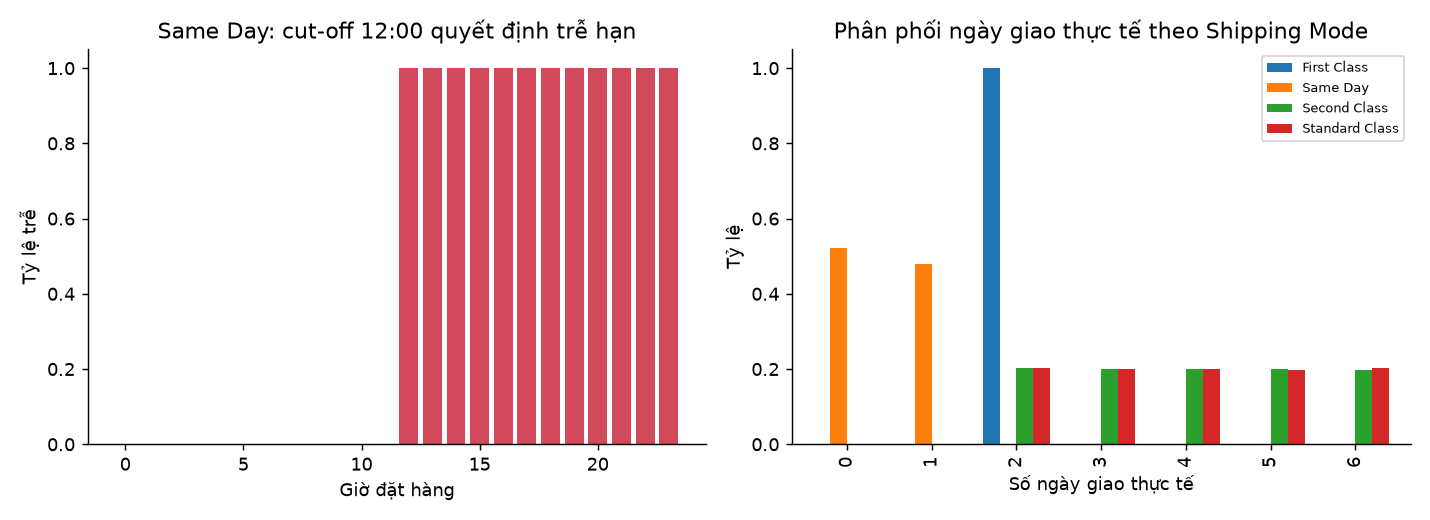
\includegraphics[width=\linewidth]{ml/06_data_generating_process.png}
\caption{Cut-off 12:00 của Same Day (trái) và phân phối ngày giao thực tế theo phương thức (phải)}
\label{fig:dgp}
\end{figure}

Từ đó xác định được \textbf{trần lý thuyết} (bộ phân loại Bayes):
\begin{equation}
P^*(\text{late}\mid x)=
\begin{cases}
1 & \text{First Class}\\
\mathbb{1}[\text{hour}\ge 12] & \text{Same Day}\\
0{,}8 & \text{Second Class}\\
0{,}4 & \text{Standard Class}
\end{cases}
\end{equation}
Mọi mô hình trung thực không thể vượt mức này một cách hệ thống; vượt quá đáng kể là dấu hiệu leakage.

% -----------------------------------------------------------------------------
\section{Thiết kế thực nghiệm}
\begin{itemize}
  \item \textbf{Out-of-time split:} train là các đơn trước 01/07/2017 (149.478 dòng), test là các đơn từ 01/07/2017 (23.287 dòng).
  \item \textbf{5-fold StratifiedGroupKFold} theo \texttt{order\_id} trên tập train: các item cùng đơn chung nhãn, nên phải chia theo nhóm.
  \item \textbf{Loại 7.754 đơn bị huỷ} khỏi train/eval (nhãn luôn bằng 0 bất kể phương thức).
  \item Tiền xử lý nằm trong sklearn \texttt{Pipeline}; chọn mô hình theo CV ROC-AUC, hoà thì theo CV Brier, không nhìn tập test.
\end{itemize}

% -----------------------------------------------------------------------------
\section{Kết quả}
\begin{table}[H]
\centering
\caption{So sánh mô hình trên tập test out-of-time (ngưỡng 0,5)}
\label{tab:model-cmp}
\small
\begin{tabular}{lrrrrcr}
\toprule
\textbf{Mô hình} & \textbf{Acc.} & \textbf{Prec.} & \textbf{Rec.} & \textbf{F1} & \textbf{ROC-AUC [95\% CI]} & \textbf{CV AUC} \\ \midrule
Baseline (tỷ lệ theo mode) & 69,90 & 89,13 & 54,45 & 0,676 & 0,750 [0,745--0,755] & 0,740 \\
Logistic Regression        & 70,98 & 89,44 & 56,33 & 0,691 & 0,754 [0,748--0,760] & 0,744 \\
\textbf{Decision Tree}     & \textbf{73,08} & \textbf{90,03} & \textbf{59,97} & \textbf{0,720} & \textbf{0,788} [0,782--0,792] & \textbf{0,774} \\
Random Forest              & 73,06 & 89,92 & 60,02 & 0,720 & 0,784 [0,778--0,789] & 0,771 \\
XGBoost                    & 72,41 & 86,59 & 61,71 & 0,721 & 0,783 [0,778--0,790] & 0,770 \\
LightGBM                   & 72,84 & 88,47 & 60,84 & 0,721 & 0,786 [0,781--0,792] & 0,771 \\ \midrule
\textit{Trần lý thuyết}    & \textit{73,08} & \textit{90,03} & \textit{59,97} & \textit{0,720} & \textit{0,781} [0,776--0,785] & \textit{0,774} \\
\bottomrule
\end{tabular}
\end{table}

\begin{figure}[H]
\centering
\begin{subfigure}{0.55\linewidth}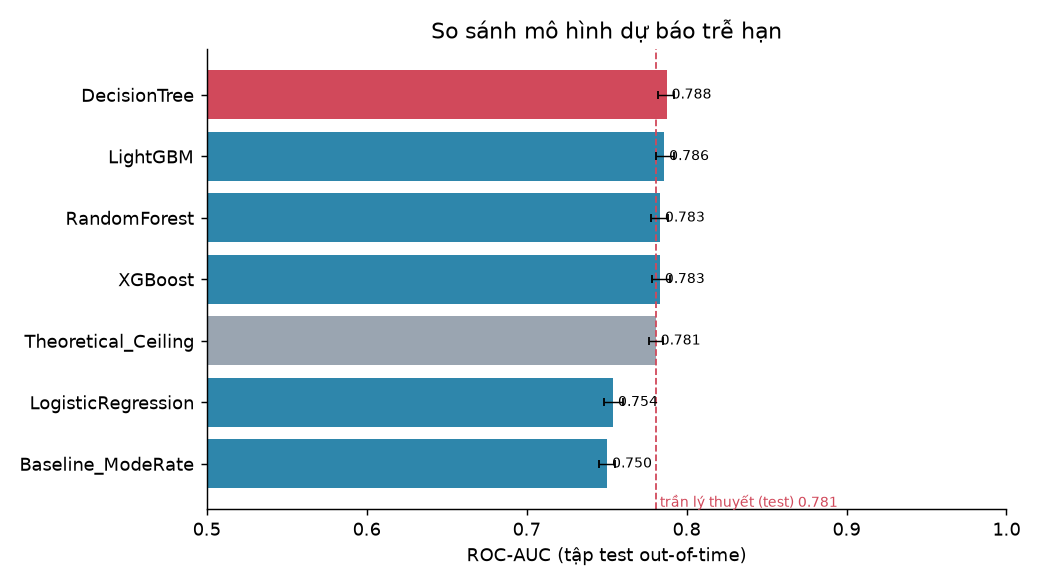
\includegraphics[width=\linewidth]{ml/01_model_comparison_auc.png}\caption{ROC-AUC kèm khoảng tin cậy}\end{subfigure}\hfill
\begin{subfigure}{0.42\linewidth}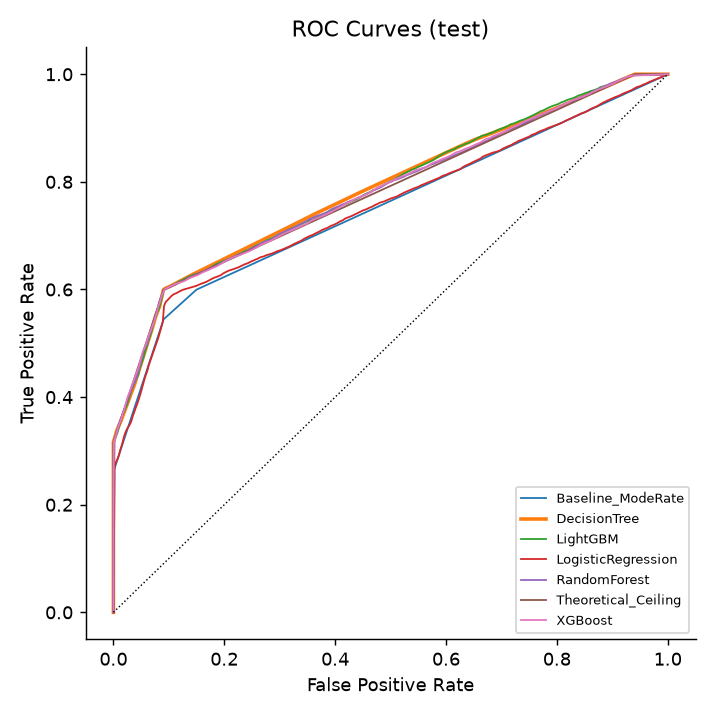
\includegraphics[width=\linewidth]{ml/02_roc_curves.png}\caption{Đường ROC}\end{subfigure}
\caption{So sánh hiệu năng các mô hình}
\label{fig:model-cmp}
\end{figure}

\paragraph{Diễn giải.}
\begin{enumerate}
  \item Các mô hình cây đều chạm trần lý thuyết. Decision Tree học đúng hai luật cốt lõi: First Class $\rightarrow$ trễ; Same Day và giờ $\ge 12$ $\rightarrow$ trễ. Các chỉ số tại ngưỡng 0,5 trùng khớp với trần.
  \item Logistic Regression kém hơn rõ rệt vì mô hình tuyến tính không học được tương tác \texttt{shipping\_mode} $\times$ \texttt{order\_hour}.
  \item Test AUC của mô hình cây nhỉnh hơn trần (0,788 so với 0,781) do dao động lấy mẫu: bên trong nhóm Standard và Second, AUC chỉ là 0,52 và 0,48. Trên CV của tập train, mô hình bằng trần (0,7743 so với 0,7736).
  \item Precision 90\% và Recall 60\%: cảnh báo ``trễ'' gần như luôn đúng, nhưng 40\% đơn trễ (chủ yếu Standard rơi vào kịch bản giao 5--6 ngày) không thể biết trước. Hạ ngưỡng xuống 0,40 thì Recall đạt 87\% và Precision 65\%.
\end{enumerate}

\begin{figure}[H]
\centering
\begin{subfigure}{0.48\linewidth}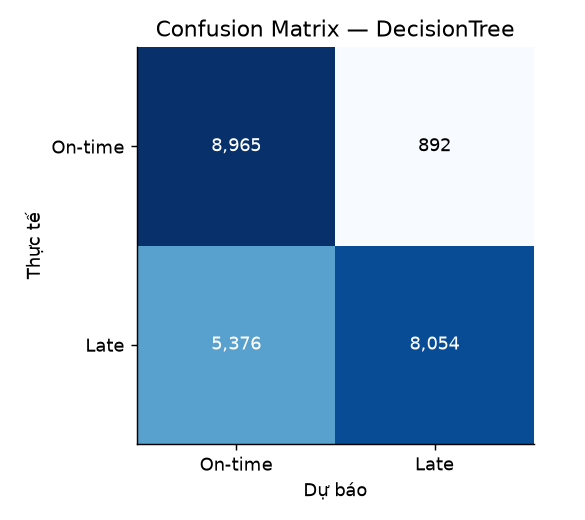
\includegraphics[width=\linewidth]{ml/03_confusion_matrix_best.png}\caption{Confusion matrix}\end{subfigure}\hfill
\begin{subfigure}{0.48\linewidth}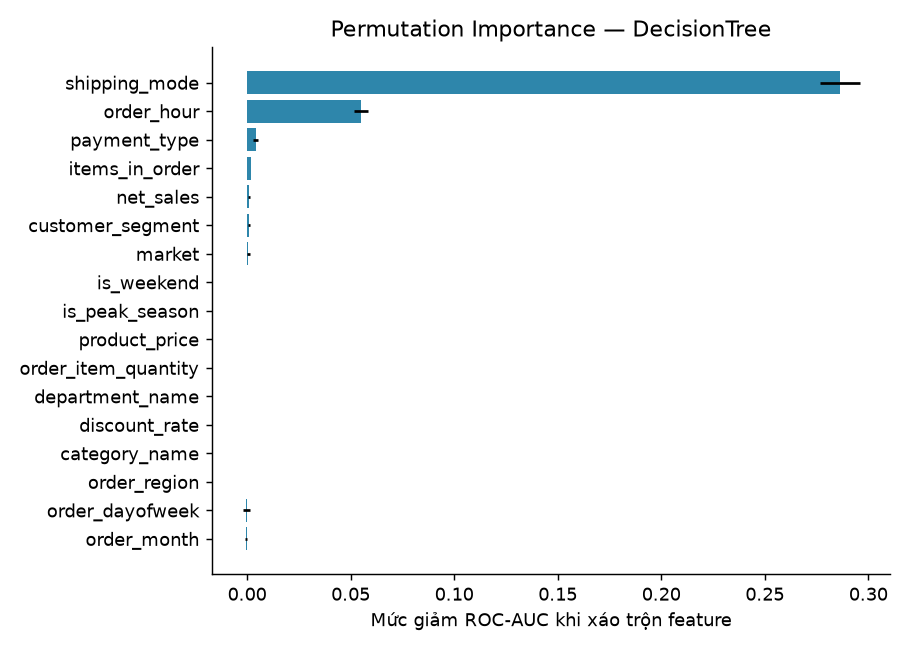
\includegraphics[width=\linewidth]{ml/04_feature_importance_best.png}\caption{Permutation importance}\end{subfigure}
\caption{Mô hình được chọn (Decision Tree)}
\label{fig:best-model}
\end{figure}

\paragraph{Yếu tố tác động.} \texttt{shipping\_mode} ($\Delta$AUC = 0,286) và \texttt{order\_hour}
(0,055) là hai yếu tố duy nhất có ý nghĩa; khu vực, ngành hàng và chiết khấu có $\Delta$AUC $<0{,}005$.
Điều này bác bỏ giả thuyết ``trễ do địa lý/sản phẩm'' và quy nguyên nhân về \textbf{chính sách SLA}.

\paragraph{Thí nghiệm leakage.} Thêm \texttt{days\_shipping\_real} vào đặc trưng cho AUC = 1,000 và
Accuracy = 100\%. Kết quả hoàn hảo nhưng vô dụng khi triển khai, minh chứng cho tầm quan trọng của
việc chọn đặc trưng pre-shipment.

% -----------------------------------------------------------------------------
\section{Feature 5 --- Dashboard đánh giá và chấm điểm rủi ro}
\todo{Chèn ảnh trang 3.1 và 3.2 vào \texttt{figures/dashboard/} và mô tả: slicer chọn mô hình, 7 KPI, ROC, importance, confusion matrix, slider ngưỡng; chấm điểm 180.519 vận đơn với 4 risk band, danh sách cảnh báo sớm.}

% -----------------------------------------------------------------------------
\section{Feature 6 --- What-If Order Delay Simulator}
Điều phối viên chọn 5 tham số (phương thức, giờ đặt, thị trường, chiết khấu, số lượng). Dashboard
tra lưới 14.400 kịch bản đã được mô hình chấm điểm trước, trả về xác suất trễ, risk band và
phương thức ít rủi ro nhất. Ví dụ: Same Day đặt lúc 14:00 có $P=100\%$, hệ thống gợi ý chuyển sang
Standard Class ($P=38\%$); đặt lúc 09:00 thì $P=0\%$.

Phần mô phỏng SLA tính tỷ lệ trễ kỳ vọng $P(\text{real days} > \text{SLA mới})$
(Bảng~\ref{tab:sla}), làm đầu vào cho Feature~8.

\begin{table}[H]
\centering
\caption{Kịch bản tái cấu trúc SLA (không tính đơn huỷ)}
\label{tab:sla}
\begin{tabular}{lccc}
\toprule
\textbf{Phương thức} & \textbf{SLA hiện tại $\rightarrow$ đề xuất} & \textbf{Trễ hiện tại} & \textbf{Trễ mới} \\ \midrule
First Class    & 1 $\rightarrow$ 2 & 100\%  & 0\% \\
Same Day       & 0 + cut-off 12:00 & 47,9\% & 0\% \\
Second Class   & 2 $\rightarrow$ 4 & 79,8\% & 39,8\% \\
Standard Class & 4 $\rightarrow$ 5 & 39,8\% & 20,2\% \\
\bottomrule
\end{tabular}
\end{table}
Áp dụng đồng thời bốn điều chỉnh, tỷ lệ trễ giảm từ 57,3\% xuống khoảng 19,8\% (OTD $\approx$ 80\%).
\todo{Chèn ảnh trang 3.3.}

% -----------------------------------------------------------------------------
\section{Hạn chế}
\begin{itemize}
  \item DataCo là dữ liệu bán tổng hợp: ngày giao của Second/Standard được sinh ngẫu nhiên đều, nên phần nhiễu này không thể khử bằng dữ liệu hiện có.
  \item Thiếu đặc trưng năng lực vận hành (hãng vận chuyển, tải kho, tuyến đường) vốn thường mang tín hiệu mạnh trong thực tế.
\end{itemize}

% ============================== CHƯƠNG 7 ==============================
\chapter{Phân tích đề xuất: Chiến lược và tối ưu lợi nhuận (Trang 4)}
\label{chap:prescriptive}

\section{Feature 7 --- Profit Erosion \& Fraud Anomaly Radar}
\todo{Phân tích Pareto 33.784 dòng lỗ ($-$3,88M USD) theo discount rate và ngành hàng; 4.062 đơn SUSPECTED\_FRAUD theo khu vực; ảnh dashboard.}

\section{Feature 8 --- SLA Re-calibration \& Financial Impact Calculator}
\todo{Dùng \texttt{data/ml/ml\_sla\_scenarios.csv} (Bảng~\ref{tab:sla}); tính tác động tài chính khi điều chỉnh SLA; ảnh dashboard.}

\section{Khuyến nghị cho doanh nghiệp}
\todo{3--5 khuyến nghị hành động có định lượng.}

% ============================== CHƯƠNG 8 ==============================
\chapter{Đánh giá hiệu năng}
\label{chap:benchmark}

\begin{table}[H]
\centering
\caption{Kết quả benchmark (\texttt{data/gold/benchmark\_performance\_report.json})}
\label{tab:bench}
\begin{tabularx}{\linewidth}{lXr}
\toprule
\textbf{Benchmark} & \textbf{Nội dung} & \textbf{Kết quả} \\ \midrule
I/O    & Đọc CSV (1.727,7 ms) so với Parquet (56,0 ms) & 30,83$\times$ \\
OLAP   & 3 truy vấn tổng hợp trên Parquet & 61,9 / 34,3 / 48,0 ms \\
Lưu trữ & CSV 91,47 MB so với Gold Parquet 6,39 MB & nén 14,31$\times$ (93\%) \\
ML     & Huấn luyện + 5-fold CV 6 mô hình & $\approx$165 s \\
\bottomrule
\end{tabularx}
\end{table}
\todo{Bổ sung PySpark vs Pandas, BigQuery bytes scanned khi có/không partition; BigQuery ML vs Python ML.}

% ============================== CHƯƠNG 9 ==============================
\chapter{Kết luận và hướng phát triển}
\label{chap:conclusion}

\section{Kết quả đạt được}
\todo{Tóm tắt: pipeline Medallion + Star Schema trên BigQuery; PySpark; 8 tính năng dashboard; mô hình dự báo đạt trần lý thuyết; phát hiện nguyên nhân trễ hạn nằm ở thiết kế SLA.}

\section{Hạn chế}
\todo{Dữ liệu bán tổng hợp; chưa streaming thời gian thực; Power BI chạy local.}

\section{Hướng phát triển}
\todo{Streaming (Pub/Sub, Dataflow), MLOps, triển khai Power BI Service, bổ sung dữ liệu hãng vận chuyển.}


\bibliographystyle{IEEEtran}
\bibliography{references}

\appendix
% ============================== PHỤ LỤC ==============================
\chapter{Hướng dẫn chạy mã nguồn}
\begin{lstlisting}[language=bash]
pip install -r requirements-ml.txt
python run_pipeline.py            # ETL: 1 -> 2 -> 2c -> 3 -> 4 -> 5 -> 6
python run_pipeline.py --step 7   # Mô hình dự báo
python dashboard/build_pbip.py    # Sinh Power BI Project
\end{lstlisting}

\chapter{Một số measure DAX tiêu biểu}
\begin{lstlisting}[language=DAX]
What-If Recommendation =
IF([What-If Is Complete],
    VAR cur = SELECTEDVALUE(ml_whatif_grid[shipping_mode])
    VAR rec = SELECTEDVALUE(ml_whatif_grid[recommended_mode])
    VAR rp  = SELECTEDVALUE(ml_whatif_grid[recommended_mode_prob])
    RETURN IF(rec = cur, "Already the lowest-risk option",
              "Switch to " & rec & " - P(late) drops to " & FORMAT(rp, "0%")),
    "Pick one value for every input")
\end{lstlisting}

\chapter{Báo cáo chất lượng dữ liệu}
\todo{Trích bảng 43 kiểm tra từ \texttt{data\_quality\_report.json}.}


\end{document}
